
We now calculate the $\WW$ production cross section according to equation \ref{eq:mainformula},

\begin{equation}
\label{eq:mainformula}
\sigma_{WW}  = \frac{N_{data} - N_{bkg}}{\epsilon \cdot {\cal{L}} \cdot BR(WW \to \ell \nu \ell \nu)}
\end{equation}

Where $N_{data}$ is the number of events observed in data, $N_{bkg}$ is the estimated number
of background events, which are summarised with their uncertainties in Table \ref{tab:data_yields}.
The distributions of the $p_{T}$ of the leading and trailing leptons, and the dilepton $p_{T}$ 
and invariant mass are shown in Figure \ref{fig:inclplots}.
The efficiency to select $\sigma_{WW \to 2\ell 2\nu}$
candidates, $\varepsilon$, is computed as the weighted mean of
the $qq\to\WW$ and $gg\to\WW$ efficiencies in simulation.
Assuming a 3\% contribution from the $gg$ process, 
$\varepsilon$ is found to be $(3.38 \pm 0.28)\%$.
The integrated luminosity of the data sample is ${\cal{L}} = $ 4920 $\pm$ 108 $\ipb$, 
and the branching ratio $BR(WW \to \ell \nu) =$ 0.1080 $\pm$ 0.0009~\cite{pdg}.

\begin{table}[ht!]
  \begin{center}
  \begin{tabular} {|c|c|}
\hline
Sample                & Yield $\pm$ stat $\pm$ syst \\ \hline \hline
$qqWW$                & 774.0 $\pm$  4.4 $\pm$ 51.0  \\ \hline
$ggWW$                & 45.9 $\pm$  0.6 $\pm$ 14.1  \\ \hline
$t\bar{t} + tW$      & 121.6 $\pm$  2.2 $\pm$ 23.3  \\ \hline
$W+jets$              & 58.3 $\pm$  3.9 $\pm$ 21.0  \\ \hline
$WZ$             & 18.5 $\pm$  0.3 $\pm$  1.8  \\ \hline
$ZZ$             & 10.6 $\pm$  0.3 $\pm$  1.8  \\ \hline
$Z/\gamma*$          & 11.7 $\pm$  3.2 $\pm$  6.0  \\ \hline
$W\gamma*/W+\gamma$ & 19.8 $\pm$  3.4 $\pm$  4.6  \\ \hline \hline
Total Bkgd.           & 241.1 $\pm$  6.5 $\pm$ 32.3  \\ \hline \hline
Total Bkgd.+Signal    & 1061.1 $\pm$  7.8 $\pm$ 62.0  \\ \hline \hline
Data                  & 1130 \\ \hline
\end{tabular}
  \caption{Expected number of signal and background events from the data-driven methods for
  an integrated luminosity of \intlumi after applying the selection requirements 
in the $\mu\mu$, $\mu{e}$, $e\mu$ and $ee$  channels.}
   \label{tab:data_yields}
  \end{center}
\end{table}

%%%%%%%%
\begin{figure}[!hbtp]
\begin{center}
\subfigure[Leading lepton $p_{T}$]{\label{subfig:fig_inclplots_pt1}
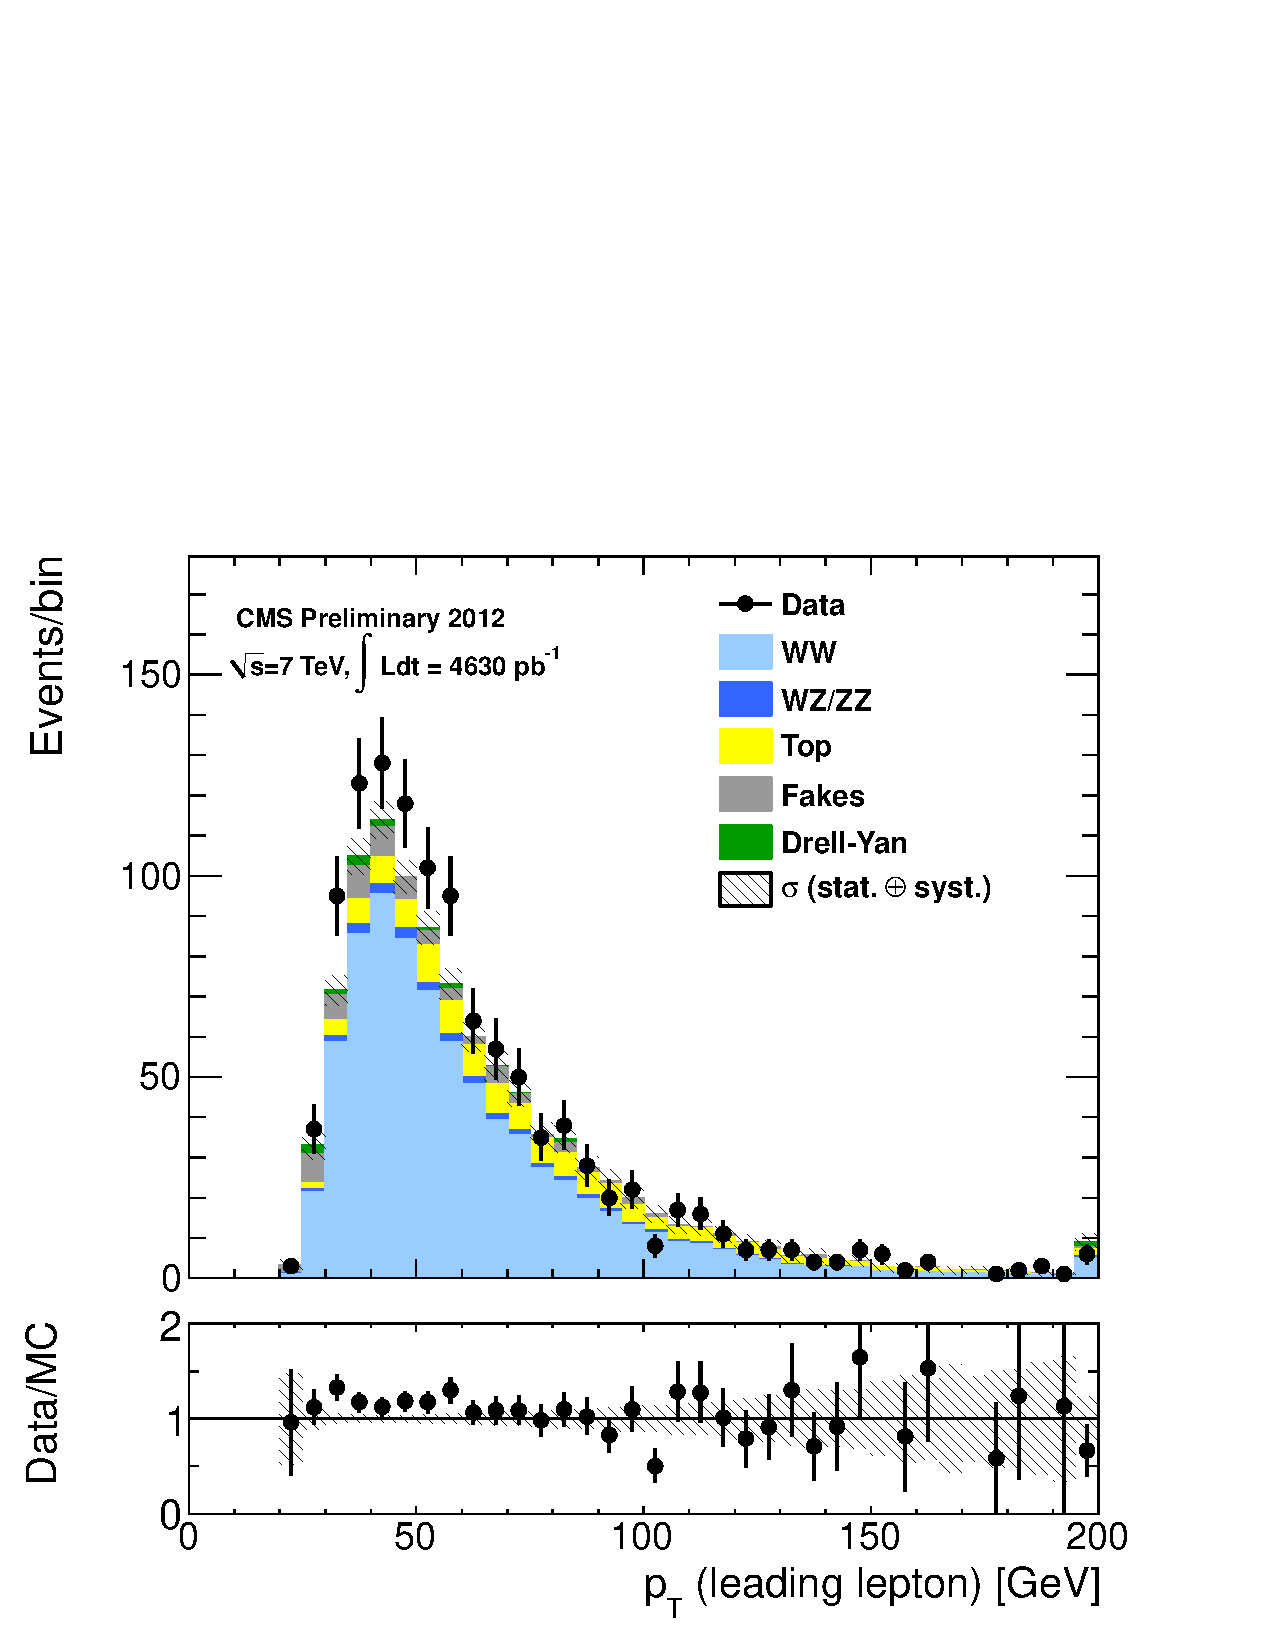
\includegraphics[width=.45\textwidth]{figures/pas_pt1_incl.pdf}}
\subfigure[Trailing lepton $p_{T}$]{\label{subfig:fig_inclplots_pt2}
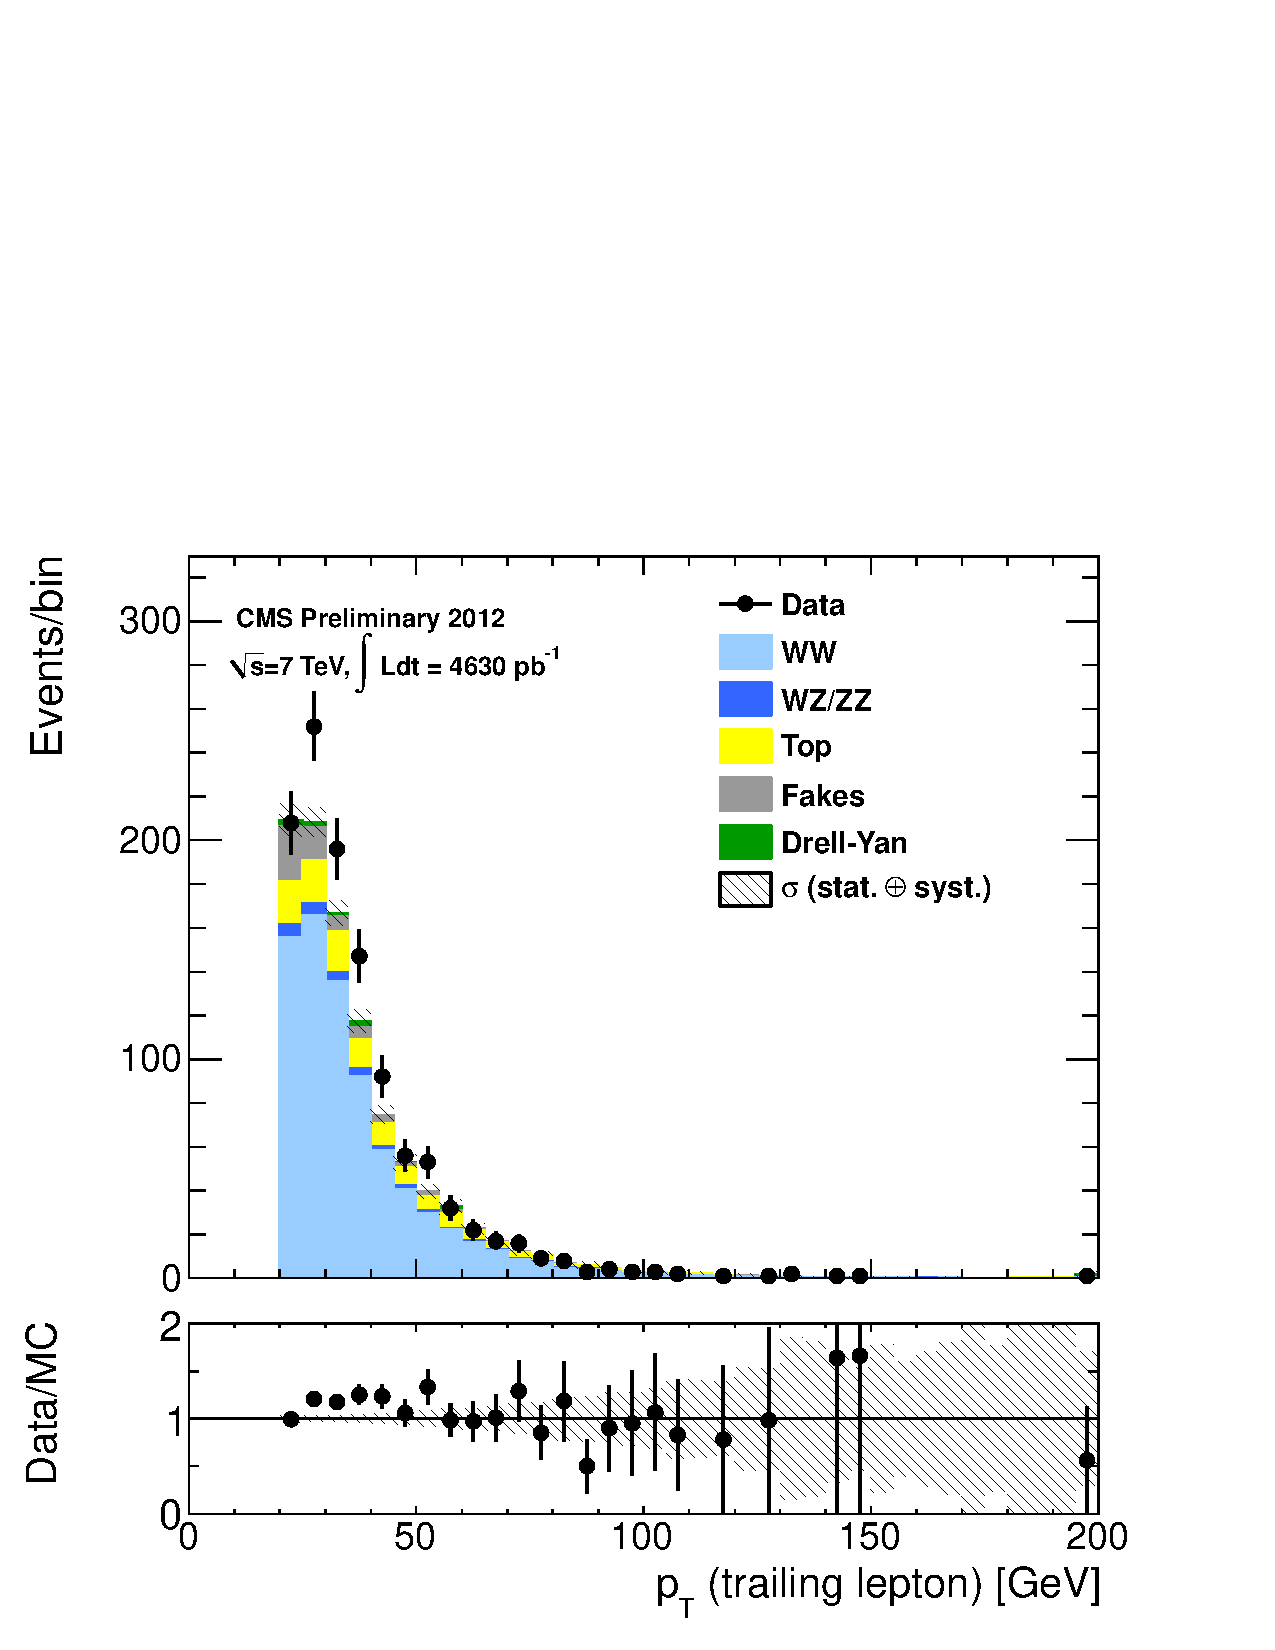
\includegraphics[width=.45\textwidth]{figures/pas_pt2_incl.pdf}}
\subfigure[Dilepton system $p_{T}$]{\label{subfig:fig_inclplots_ptll}
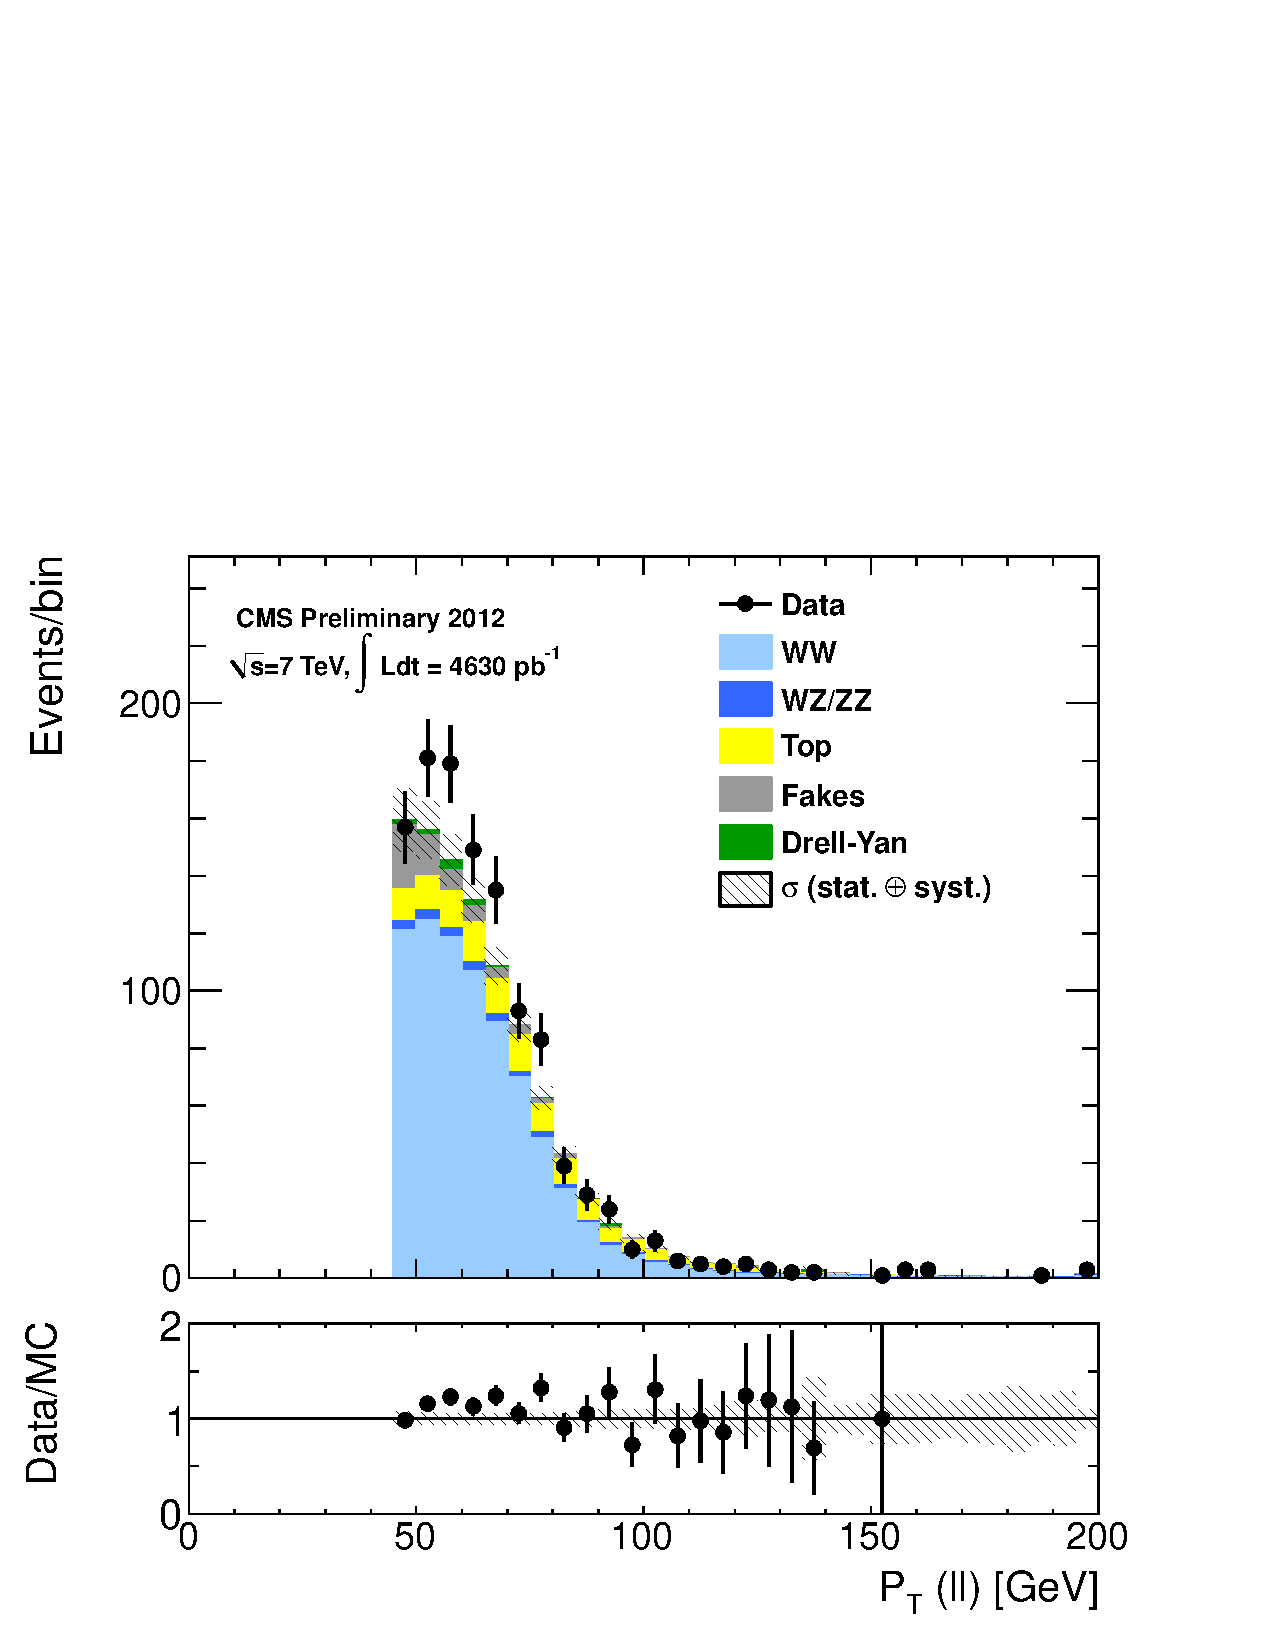
\includegraphics[width=.45\textwidth]{figures/pas_ptll_incl.pdf}}
\subfigure[Dilepton system invariant mass]{\label{subfig:fig_inclplots_M}
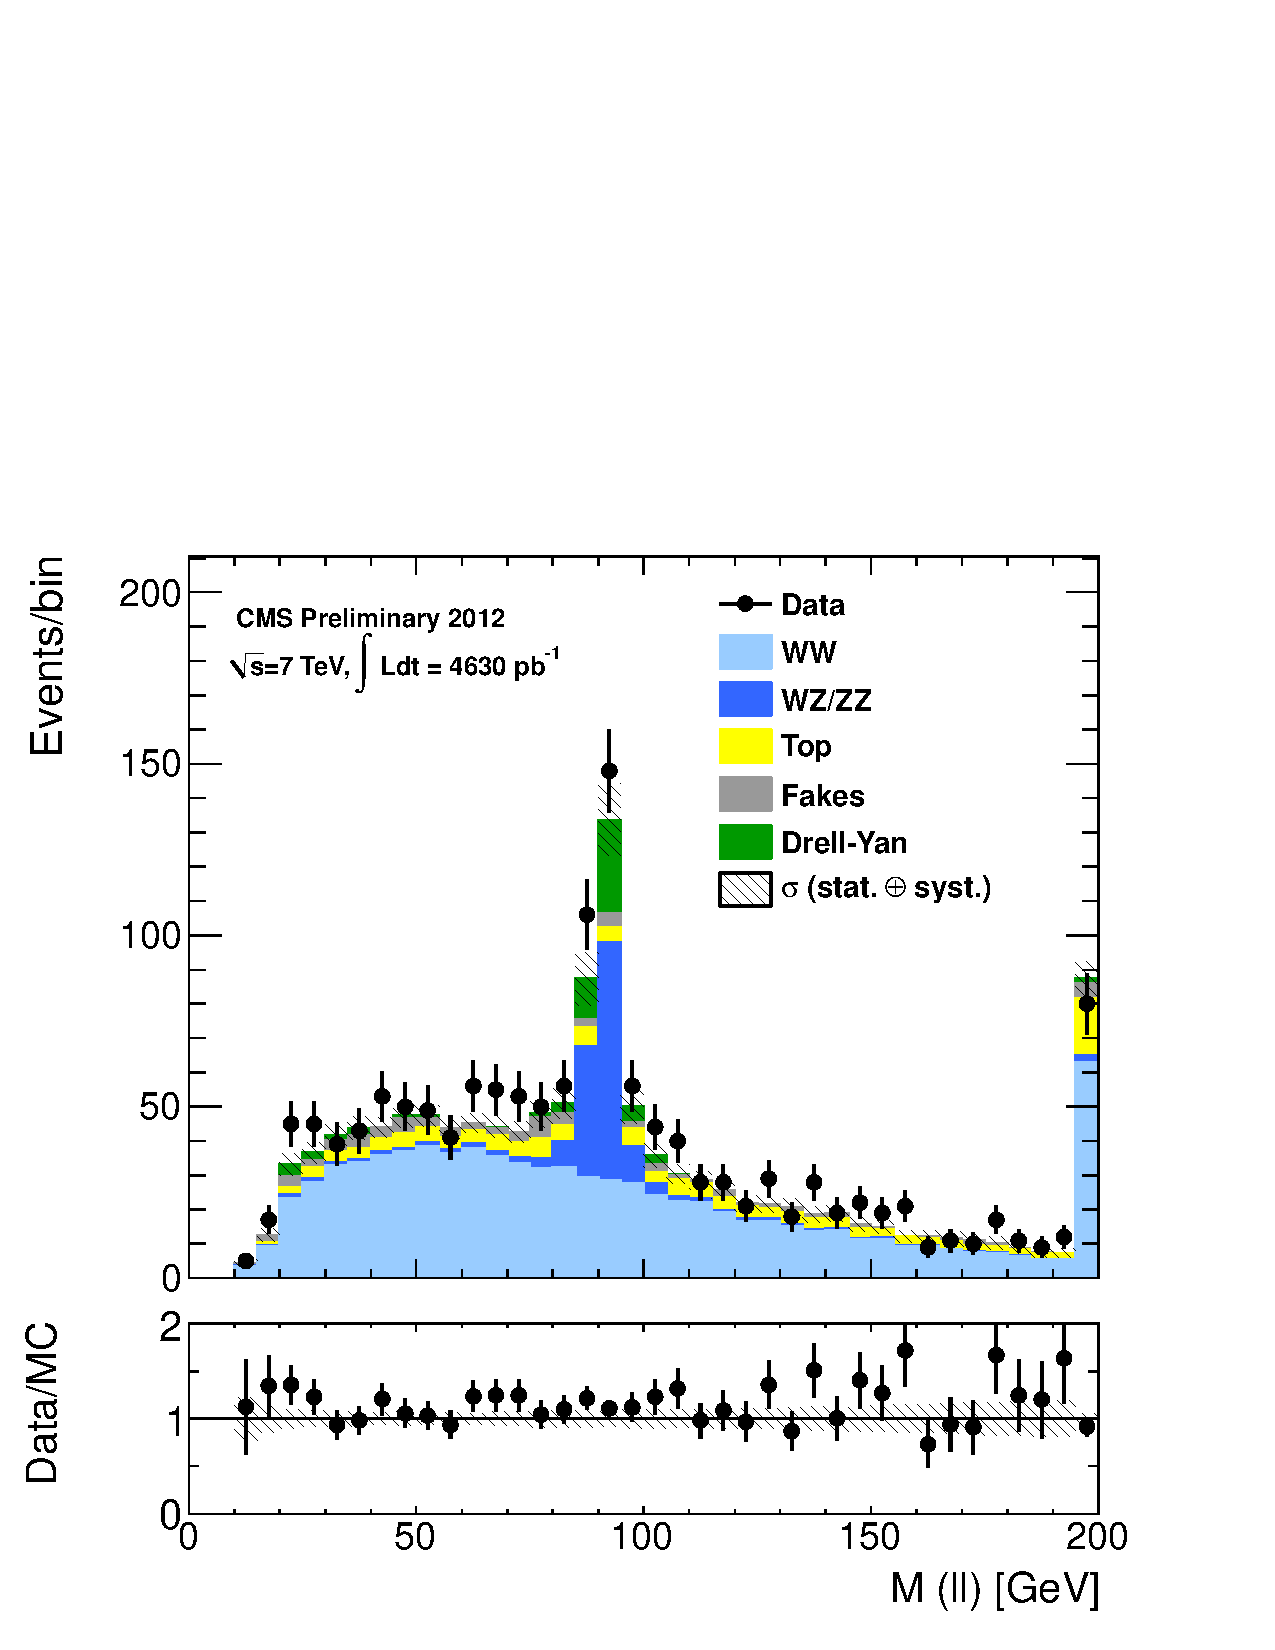
\includegraphics[width=.45\textwidth]{figures/pas_mll_incl.pdf}}
\caption{Kinematic distributions for expected and observed events in the  $\mu\mu$, $\mu{e}$, $e\mu$ and $ee$ channels.
The dilepton system invariant mass distribution has the $Z$ mass veto relaxed.
The uncertainty on the expected events includes both statistical and systematic components.}
\label{fig:inclplots}
\end{center}
\end{figure}
%%%%%%%%


Using the inputs described previously and Equation \ref{eq:mainformula},
we obtain the following $WW$ cross-section measurement:

\begin{equation*}
\sigma_{WW}  = 50.95 \pm 1.93~\mathrm{(stat.)} \pm 4.45~\mathrm{(syst.)} \pm 1.12~\mathrm{(lumi.)~pb}.
\end{equation*}

The cross section obtained in each dilepton channel is documented in Appendix \ref{sec:xsec_per_channel}.

